\chapter{Literature Review}\label{cha:literature}

\section{State of the Art}

    \subsection{ROS on Web}

        The closest representation of the intended project is the work produced by Michael Allwright known as \textit{ROS on Web}. Allwright shares the same goal as the author to develop the technology which allows for running ROS nodes entirely on the browser by cross-compiling C++ code to WebAssembly and using web workers to handle the internal communication~\cite{rosonweb}.

        Equivalently, Allwright targeted the \ac{ROS} 2 distribution. It is suspected that the \textit{galactic} version was used for the demonstrations. The main demonstration of a running publisher and subscriber is illustrated in Figure~\ref{fig:rosweb}.
        
        
        \begin{figure}[htbp]
            \centering
            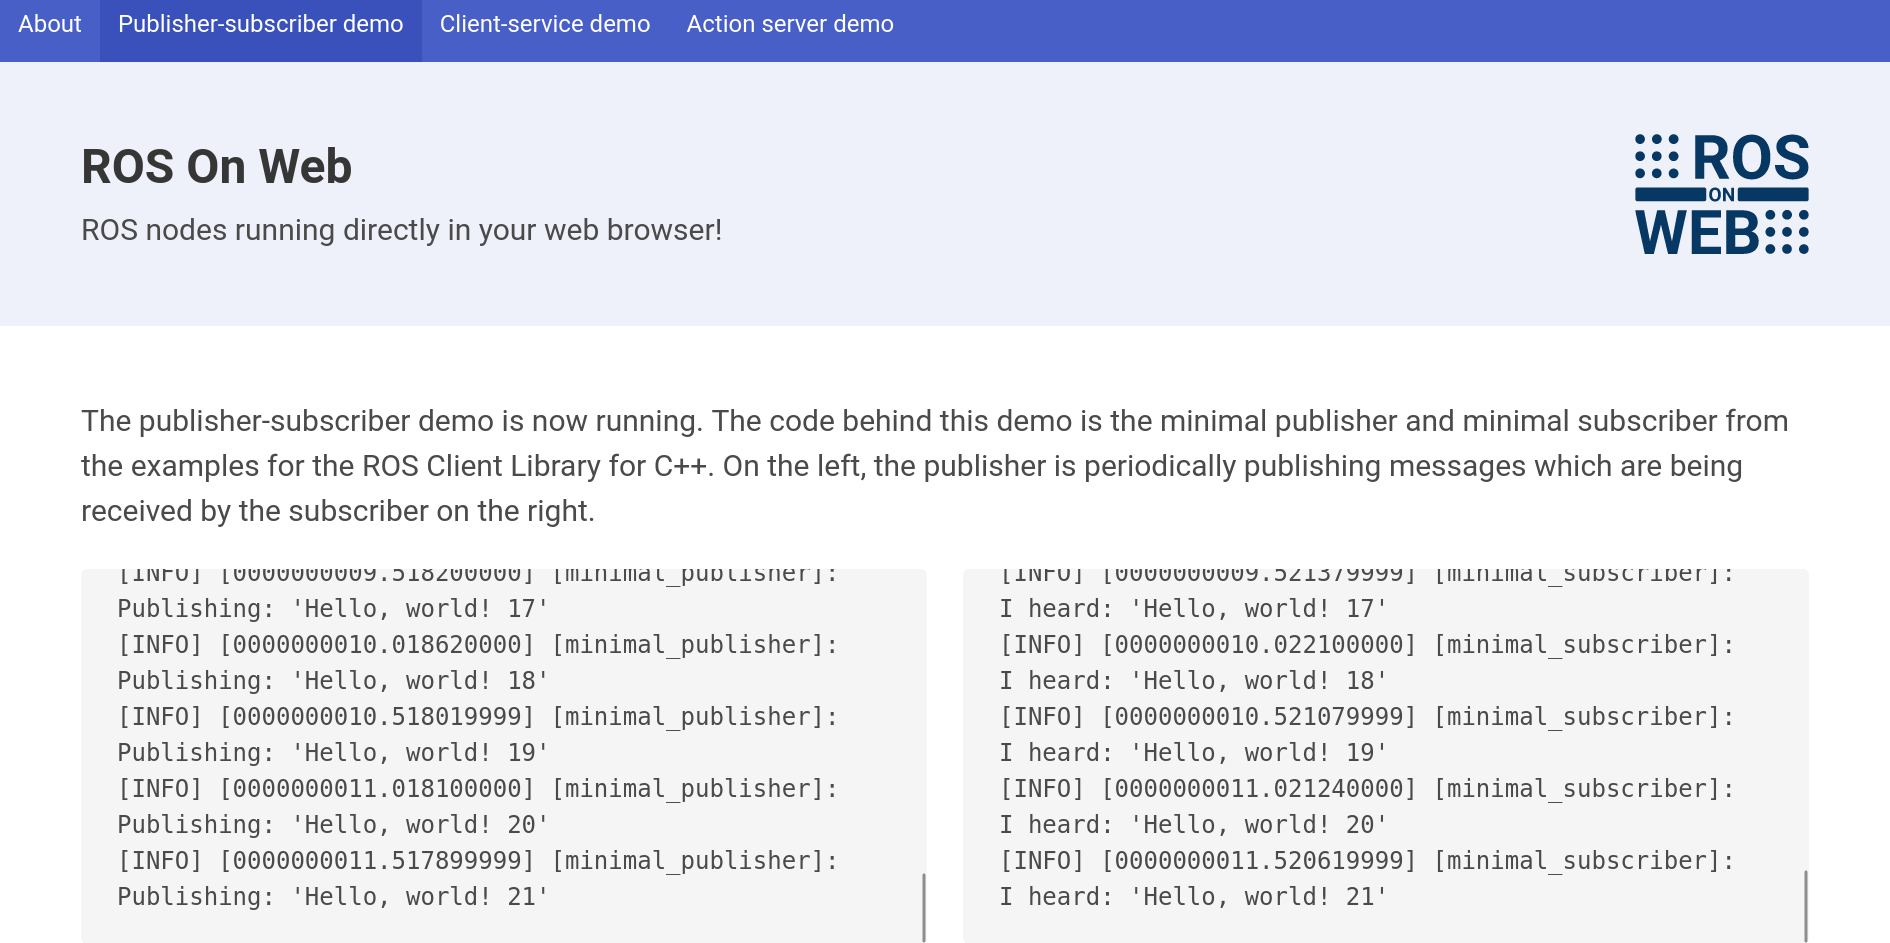
\includegraphics[width=\textwidth]{01_rosOnWeb.png}
            \caption{\textit{ROS on Web} publisher and subscriber demonstration.}
            \label{fig:rosweb}
        \end{figure}

        Nonetheless, the greatest disadvantage of \textit{ROS on Web} lies in the fact that the project is not open source. Very little can be derived about how Allwright was able to achieve the demonstrations represented on the website. A few hints are given in the introductory page such as the replacement of the middleware with a custom design and the use of web workers. However, it is not possible to determine the manner in which these technologies were used. Hope remains that in the near future, the repositories for \textit{ROS on Web} become publicly available as an extension of the ROS open source ecosystem.


\section{Relevant Works}

    \subsection{ROSbridge}

    \subsection{ROS Control Center}

    \subsection{ROSboard}

    \subsection{ROSlink}

    \subsection{Foxglove Studio}
        % https://foxglove.dev/blog/publishing-and-visualizing-ros2-transforms

        \begin{figure}[htbp]
            \centering
            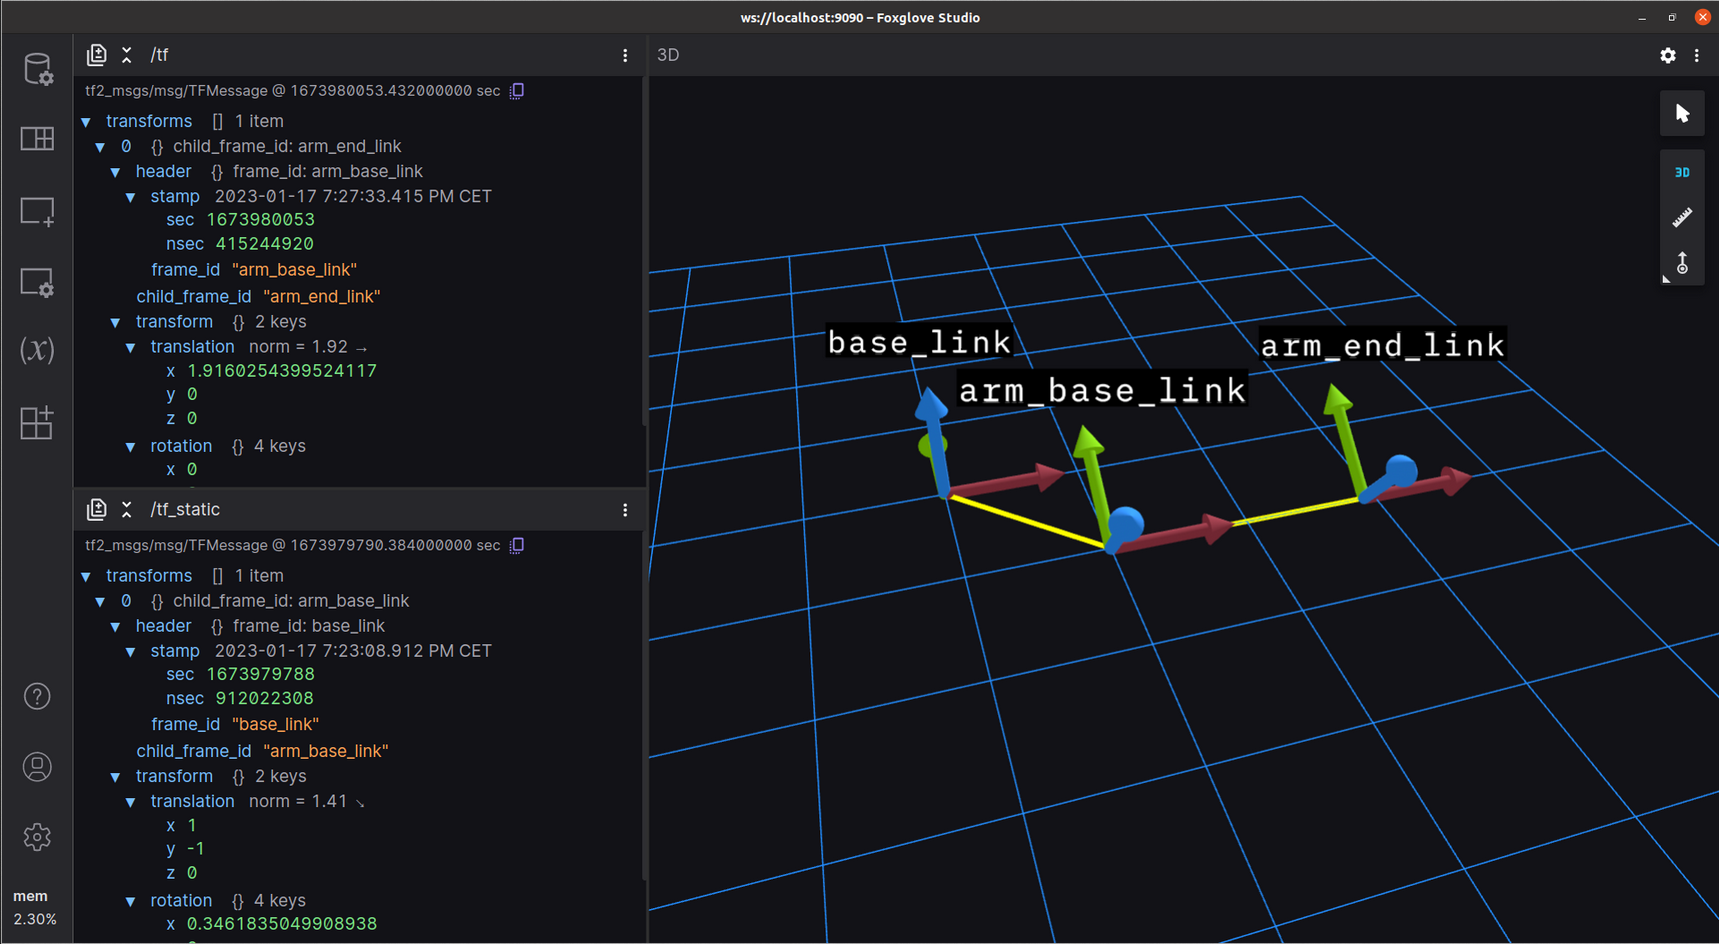
\includegraphics[width=\textwidth]{01_FoxgloveStudio.png}
            \caption{Visualizing ROS 2 Transforms with Foxglove Studio}
        \end{figure}

\section{State of WASM}

    \subsection{Unity in WebAssembly}

    % https://blog.unity.com/technology/webassembly-is-here
    % https://beta.unity3d.com/jonas/AngryBots/

    \begin{figure}[htbp]
        \centering
        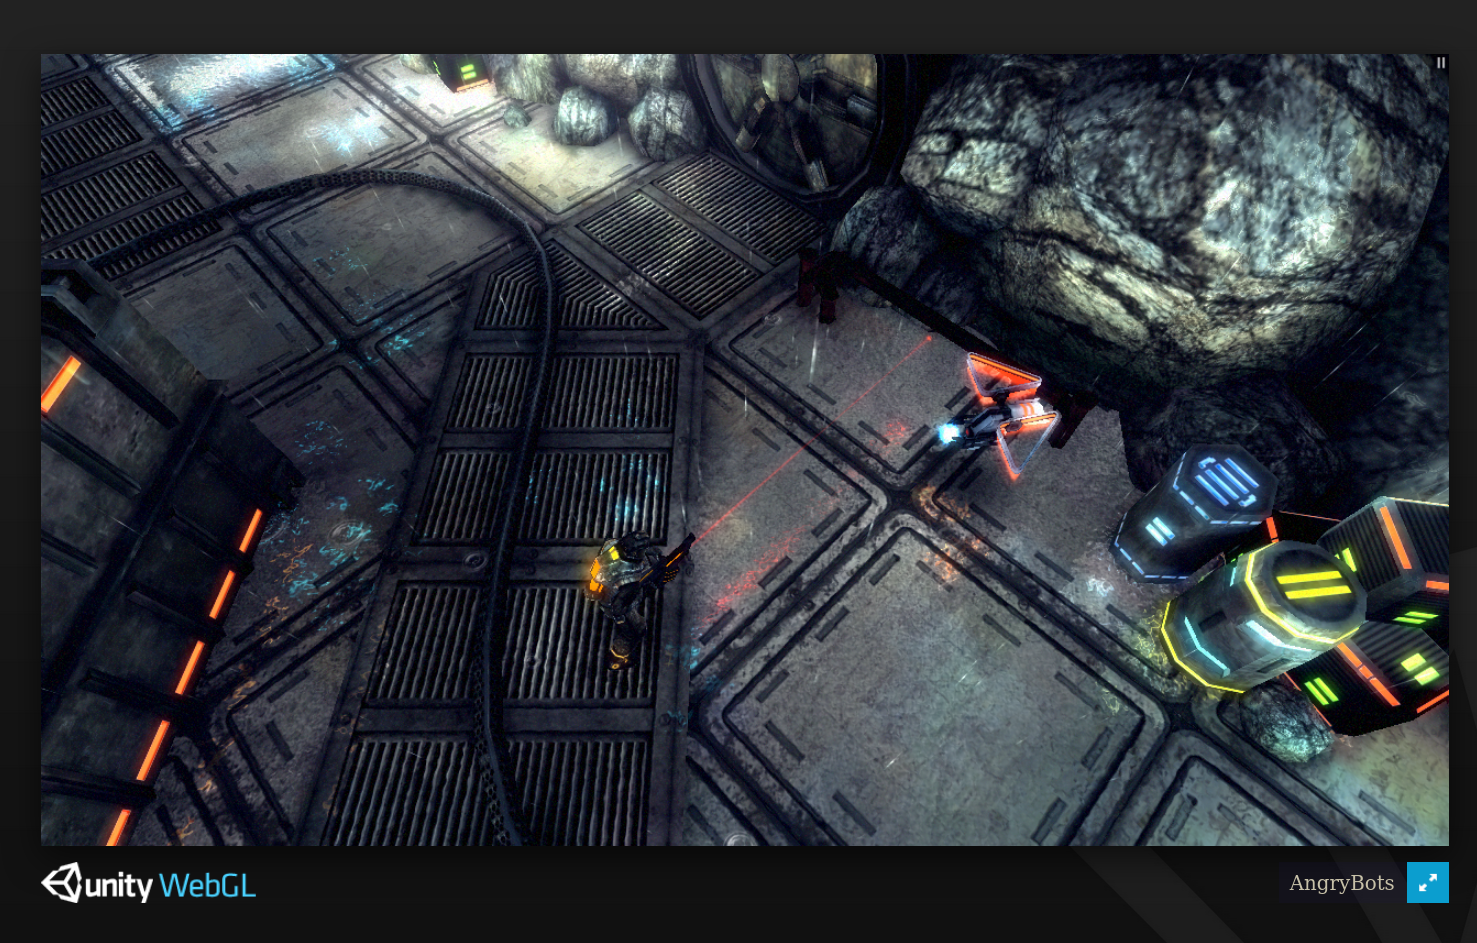
\includegraphics[width=0.8\textwidth]{01_angryBots.png}
        \caption{Demo of Angry Bots in Unity WebGL}\label{fig:unity}
    \end{figure}
